\chapter{Final edges at vertices of high degree}\label{sec:high}

This section proves \cref{thm:high-main}, the estimate for final edges at vertices of degree greater than $D_n$ required by \cref{prop:red-split}. It bounds the probability that the process becomes non-colorable by time $M$ through a final edge $e_H$ with an endpoint of degree greater than $D_n$ in $\Gamma$. The bound requires no restriction on the expected lifetime $r(\Gamma)$. Since it concerns all final edges up to time $M$, it also bounds, for all integers $0 \le L' \le U' \le M$, the probability that $L' < H \le U'$ and both endpoints of $e_H$ have degree greater than $D_n$ in $\Gamma$. The heuristics behind the argument are explained in \cref{sec:overview}. The arguments use the number of colors only through the notion of colorability, and they hold for $q = 2$ as well (see \cref{rem:high-q2}).

The argument has three steps. In \cref{sec:high-pivotal}, we delete edge occurrences and record whether two specified vertices must still receive the same color in every coloring. Iterating the estimate for deletions that preserve this equality reduces the high-degree probability to the density of pairs for which many incident deletions destroy the equality (\cref{prop:high-descent}). We express this density through a relation, defined below, that records possible additions to the frozen class of a vertex (\cref{lem:high-deletion}). In \cref{sec:high-relation}, we bound the density of this relation by the expected value of a logarithmic increment defined below (\cref{lem:high-onestep}). This increment is also defined when the added edge makes the graph non-colorable. In \cref{sec:high-potential}, we compare these increments with the growth of the logarithm of the frozen-class size before the last step and bound the last increment separately. Their sum is bounded by $\log n$, which controls the expected sum of the relation densities after a stopping time (\cref{thm:high-potential}). Finally, \cref{sec:high-main} combines this estimate with a binomial tail bound for the probability that a fixed vertex reaches the required degree by time $M$.

Throughout this section, $n \ge 3$, and $\Lambda > 0$ and $M = \lfloor \Lambda n \rfloor$ are as in \cref{sec:pre-process}; the results of this section use only $\Lambda > 0$. Recall the degree cut $D_n = \lfloor (\log n)^{1/4} \rfloor$ from \eqref{eq:red-parameters}. We set
\begin{equation}\label{eq:high-params}
K = \lceil 8 \Lambda \rceil, \qquad w_0 = \lfloor D_n / 2 \rfloor.
\end{equation}
Since $n \ge 3$, we have $D_n \ge 1$ and therefore $0 \le w_0 < D_n$. For distinct vertices $a$ and $b$, we let $ab$ denote the pair $\{a, b\}$. Recall that the degree $\deg_G(u)$ counts occurrences with multiplicity, that the relation $u \sim_G v$ includes the requirement that $G$ is colorable, and that every quantity defined through colorings or frozen classes is set to zero on non-colorable multigraphs.

\section{Pivotal occurrences}\label{sec:high-pivotal}

We first define the two kinds of occurrences at an endpoint of a frozen pair.

\begin{definition}\label{def:high-pivotal}
Let $G$ be a colorable multigraph on $[n]$, and let $(u, v)$ be an ordered pair of distinct vertices such that $u \sim_G v$. We call $(u, v)$ an \emph{ordered frozen pair} of $G$. Let $e$ be an occurrence of $G$ with $u \in e$. We say that $e$ is \emph{non-pivotal} for $(u, v)$ if $u \sim_{G - e} v$, and that $e$ is \emph{pivotal} for $(u, v)$ otherwise. For an integer $j \ge 0$, we define
\begin{equation}\label{eq:high-kappaj}
\kappa_j(G) = \frac{1}{n(n - 1)} \, \# \bigl\{ (u, v) \in [n]^2 : u \ne v, \ u \sim_G v, \ \deg_G(u) = j \bigr\},
\end{equation}
and we define $\kappa_j^{\rm np}(G)$ by the same formula, with the additional requirement that at least $K$ of the $j$ occurrences at $u$ are non-pivotal for $(u, v)$. We set $\kappa_j^{\rm piv}(G) = \kappa_j(G) - \kappa_j^{\rm np}(G)$. If $G$ is not colorable, we set $\kappa_j(G) = \kappa_j^{\rm np}(G) = \kappa_j^{\rm piv}(G) = 0$.
\end{definition}

Occurrences are counted with multiplicity, so that exactly $\deg_G(u)$ occurrences contain $u$. Note that $G - e \subset G$ is colorable. Moreover, $G - e$ is determined by the pair $e$ and not by the occurrence that is removed. All occurrences of a pair are pivotal or all are non-pivotal. An occurrence of a pair of multiplicity at least two is non-pivotal, since $G - e$ then has the same colorings as $G$.

A pair counted in $n(n - 1) \kappa_j^{\rm piv}(G)$ has at least $j - K + 1$ pivotal occurrences at $u$. By \cref{lem:pre-frozen}(a), applied to the colorable multigraph $G - e$, the occurrence $e$ is non-pivotal for $(u, v)$ if and only if $(G - e) + uv$ is not colorable. Thus $e$ is pivotal for $(u, v)$ exactly when it is pivotal, in the usual sense \cite[Section~2, p.~130]{russo1982approximate}, for the increasing event that $G + uv$ is not colorable, in the sense that $G$ belongs to this event and $G - e$ does not (see \cite[Section~4.8, Exercise~4.9]{grimmett2018probability}).

We will also need a relation that records how the frozen class of a vertex grows when an edge at that vertex is added.

\begin{definition}\label{def:high-relation}
Let $G$ be a colorable multigraph on $[n]$, let $u \in [n]$, and let $W = [n] \setminus C_G(u)$. We define $R_G(u)$ to be the set of ordered pairs $(y, v) \in W \times W$ such that
\begin{equation}\label{eq:high-R}
\sigma(u) \in \{ \sigma(y), \sigma(v) \} \qquad \text{for all } \sigma \in \Col(G).
\end{equation}
For $y \in [n]$, we define the \emph{section} $R_G(u; y) = \{ v \in [n] : (y, v) \in R_G(u) \}$, and we set
\begin{equation}\label{eq:high-beta}
\beta_G(u) = n^{-2} \abs{R_G(u)}.
\end{equation}
If $G$ is not colorable, we set $R_G(u) = \emptyset$ and $\beta_G(u) = 0$.
\end{definition}

Equivalently, $\beta_G(u)$ is the probability that two independent uniform vertices $y$ and $v$ of $[n]$ lie outside $C_G(u)$ and that every coloring of $G$ gives $u$ the color of $y$ or the color of $v$. The section $R_G(u; y)$ is empty for $y \in C_G(u)$. When $G$ and $u$ are fixed, we let $R(y)$ denote $R_G(u; y)$. In this notation, we let $W$ denote $[n] \setminus C_G(u)$.

\begin{lemma}\label{lem:high-relation}
Let $G$ be a colorable multigraph on $[n]$ and let $u \in [n]$.
\begin{enumerate}[label=(\alph*)]
\item The relation $R_G(u)$ is symmetric, and $(y, y) \notin R_G(u)$ for all $y \in [n]$.
\item For all $y \in W$, the multigraph $G + uy$ is colorable and $C_{G + uy}(u) = C_G(u) \cup R(y)$.
\end{enumerate}
\end{lemma}

\begin{proof}
For (a), note that the condition \eqref{eq:high-R} is symmetric in $y$ and $v$. For $v = y$, it states that $\sigma(u) = \sigma(y)$ for all colorings $\sigma$ of $G$, which means that $y \in C_G(u)$ and is excluded by the requirement $y \in W$.

For (b), let $y \in W$. We have $y \ne u$ and $u \not \sim_G y$, and \cref{lem:pre-frozen}(a) implies that $G + uy$ is colorable. The colorings of $G + uy$ are the colorings $\sigma$ of $G$ with $\sigma(y) \ne \sigma(u)$. Therefore $v \in C_{G + uy}(u)$ if and only if every coloring $\sigma$ of $G$ with $\sigma(y) \ne \sigma(u)$ satisfies $\sigma(v) = \sigma(u)$, which gives
\[
v \in C_{G + uy}(u) \iff \sigma(u) \in \{ \sigma(y), \sigma(v) \} \quad \text{for all } \sigma \in \Col(G).
\]
The right side holds for all $v \in C_G(u)$, and for $v \in W$ it is the condition $(y, v) \in R_G(u)$.
\end{proof}

By \cref{lem:high-relation}(b), for $y \in W$, the number $\abs{R(y)}$ counts the vertices that join the frozen class of $u$ when the pair $uy$ is added to $G$. Since $\abs{R_G(u)} = \sum_{y \in [n]} \abs{R(y)}$, the quantity $n \beta_G(u)$ is the average of $\abs{R(y)}$ over $y \in [n]$.

We now bound the densities $\kappa_j^{\rm np}$ and $\kappa_j^{\rm piv}$ of \cref{def:high-pivotal} in terms of graphs with one occurrence fewer. To that end, we remove one of the $m$ occurrences $e_1, \dots, e_m$ of $G_m$. For each $i \le m$, the multigraph $G_m - e_i$ is formed by the $m - 1$ independent uniform pairs $e_{i'}$ with $i' \ne i$, which are also independent of $e_i$. The pair $(G_m - e_i, e_i)$ therefore has the law of $(G_{m - 1}, e)$, where $e$ is a uniform pair independent of $G_{m - 1}$, and for every function $h \ge 0$ of a multigraph and a pair we have
\begin{equation}\label{eq:high-exchange}
\E \sum_{i = 1}^m h(G_m - e_i, e_i) = m \E h(G_{m - 1}, e).
\end{equation}
This is the analogue for $m$ independent points of the Mecke equation for Poisson processes \cite{mecke1967stationare}, \cite[Theorem~4.1]{last2018lectures}.

\begin{lemma}\label{lem:high-deletion}
Let $m \ge 1$ and $j \ge 1$ be integers.
\begin{enumerate}[label=(\alph*)]
\item We have
\begin{equation}\label{eq:high-deletion-np}
\E \kappa_j^{\rm np}(G_m) \le \frac{2m}{nK} \, \E \kappa_{j - 1}(G_{m - 1}).
\end{equation}
\item If $j \ge K$, then for all $u \in [n]$,
\begin{equation}\label{eq:high-deletion-piv}
\E \kappa_j^{\rm piv}(G_m) \le \frac{2mn}{(n - 1)^2 (j - K + 1)} \, \E \bigl[ \ind \{ \deg_{G_{m - 1}}(u) = j - 1 \} \, \beta_{G_{m - 1}}(u) \bigr].
\end{equation}
\end{enumerate}
\end{lemma}

\begin{proof}
We begin with (a). For a multigraph $G'$ and a pair $e$, we define $h_1(G', e)$ by
\[
h_1(G', e) = \sum_{a \in e} \sum_{v \in [n] \setminus \{a\}} \ind \bigl\{ a \sim_{G' + e} v, \ a \sim_{G'} v, \ \deg_{G' + e}(a) = j \bigr\}.
\]
Let $(a, v)$ be a pair counted in $n(n - 1) \kappa_j^{\rm np}(G_m)$. Then $a \sim_{G_m} v$, $\deg_{G_m}(a) = j$, and there exist at least $K$ indices $i \le m$ such that $a \in e_i$ and $a \sim_{G_m - e_i} v$. Each such index contributes $1$ to $h_1(G_m - e_i, e_i)$, through the endpoint $a$ and the vertex $v$. Summing over the pairs $(a, v)$ and taking expectations, we obtain
\begin{equation}\label{eq:high-deletion-1}
K n (n - 1) \E \kappa_j^{\rm np}(G_m) \le \E \sum_{i = 1}^m h_1(G_m - e_i, e_i) = m \E h_1(G_{m - 1}, e),
\end{equation}
where the identity is \eqref{eq:high-exchange}.

We now bound the right side of \eqref{eq:high-deletion-1}. For $a \in e$, we have $\deg_{G_{m - 1} + e}(a) = \deg_{G_{m - 1}}(a) + 1$. Recall from \cref{sec:pre-process} that each vertex belongs to $e$ with probability $2/n$, and note that $e$ is independent of $G_{m - 1}$. Dropping the first indicator in the definition of $h_1$, we find
\[
\begin{split}
\E h_1(G_{m - 1}, e) &\le \E \sum_{a \in e} \sum_{v \in [n] \setminus \{a\}} \ind \bigl\{ a \sim_{G_{m - 1}} v, \ \deg_{G_{m - 1}}(a) = j - 1 \bigr\}\\
&= \frac{2}{n} \sum_{a \in [n]} \sum_{v \in [n] \setminus \{a\}} \Pp \bigl( a \sim_{G_{m - 1}} v, \ \deg_{G_{m - 1}}(a) = j - 1 \bigr)\\
&= \frac{2}{n} \, n (n - 1) \E \kappa_{j - 1}(G_{m - 1}),
\end{split}
\]
where in the last step we used the definition \eqref{eq:high-kappaj}. Inserting this bound into \eqref{eq:high-deletion-1} gives \eqref{eq:high-deletion-np}.

We now prove (b). Let $(a, v)$ be a pair counted in $n(n - 1) \kappa_j^{\rm piv}(G_m)$. At most $K - 1$ of the $j$ occurrences at $a$ are non-pivotal for $(a, v)$, so there exist at least $j - K + 1$ indices $i \le m$ such that $a \in e_i$ and $a \not \sim_{G_m - e_i} v$. Further, $\deg_{G_m - e_i}(a) = j - 1$ for these indices.

We set
\[
h_2(G', e) = \sum_{a \in e} \sum_{v \in [n] \setminus \{a\}} \ind \bigl\{ a \sim_{G' + e} v, \ a \not \sim_{G'} v, \ \deg_{G'}(a) = j - 1 \bigr\}.
\]
Each index $i$ as above contributes $1$ to $h_2(G_m - e_i, e_i)$, and as in the proof of (a), we obtain
\begin{equation}\label{eq:high-deletion-2}
(j - K + 1) \, n (n - 1) \E \kappa_j^{\rm piv}(G_m) \le m \E h_2(G_{m - 1}, e).
\end{equation}

To compute the right side of \eqref{eq:high-deletion-2}, we condition on $G' = G_{m - 1}$. We may assume that $G'$ is colorable, since otherwise $h_2(G', e) = 0$. Let $a$ and $y$ be distinct vertices. We claim that
\begin{equation}\label{eq:high-deletion-3}
\sum_{v \in [n] \setminus \{a\}} \ind \bigl\{ a \sim_{G' + ay} v, \ a \not \sim_{G'} v \bigr\} = \abs{R_{G'}(a; y)}.
\end{equation}
Indeed, suppose first that $y \in C_{G'}(a)$. Then $G' + ay$ is not colorable by \cref{lem:pre-frozen}(a), the left side vanishes, and $R_{G'}(a; y) = \emptyset$ by \cref{def:high-relation}. Otherwise, \cref{lem:high-relation}(b) shows that the vertices $v$ counted on the left are exactly the elements of $R_{G'}(a; y)$.

Every pair $ay$ has probability $\binom{n}{2}^{-1}$, and summing over the two endpoints of $e$ amounts to summing over ordered pairs $(a, y)$. Using \eqref{eq:high-deletion-3} and $R_{G'}(a; a) = \emptyset$, we obtain
\[
\begin{split}
\E \bigl[ h_2(G', e) \bigm| G' \bigr] &= \binom{n}{2}^{-1} \sum_{a \in [n]} \ind \{ \deg_{G'}(a) = j - 1 \} \sum_{y \in [n] \setminus \{a\}} \abs{R_{G'}(a; y)}\\
&= \binom{n}{2}^{-1} \sum_{a \in [n]} \ind \{ \deg_{G'}(a) = j - 1 \} \, \abs{R_{G'}(a)}\\
&= \frac{2n}{n - 1} \sum_{a \in [n]} \ind \{ \deg_{G'}(a) = j - 1 \} \, \beta_{G'}(a),
\end{split}
\]
where in the last step we used \eqref{eq:high-beta}. Recall that the law of $G_{m - 1}$ is invariant under relabeling. Relabeling $G$ and $a$ by the same permutation does not change $\ind \{ \deg_G(a) = j - 1 \} \beta_G(a)$. Every term of the last sum has the same expectation. For all $u \in [n]$, we have
\[
\E h_2(G_{m - 1}, e) = \frac{2n^2}{n - 1} \, \E \bigl[ \ind \{ \deg_{G_{m - 1}}(u) = j - 1 \} \, \beta_{G_{m - 1}}(u) \bigr].
\]
Inserting this identity into \eqref{eq:high-deletion-2} and dividing by $(j - K + 1) n (n - 1)$, we arrive at \eqref{eq:high-deletion-piv}.
\end{proof}

We now iterate \cref{lem:high-deletion}(a). Recall that $K = \lceil 8 \Lambda \rceil$, so that the coefficient in \eqref{eq:high-deletion-np} satisfies $2m/(nK) \le 1/4$ for $m \le M$. Each application lowers the degree and the time by one. After $j - w_0$ applications, the term $\E \kappa_j(G_m)$ with $j > D_n$ is bounded by $4^{-(j - w_0)} \E \kappa_{w_0}(G_{m - j + w_0})$ plus a combination of the terms $\E \kappa_{j'}^{\rm piv}$ with $j' > w_0$; see \eqref{eq:high-iterate} below. The terms of the first kind are controlled by \cref{lem:pre-hazard}, which uses that the process becomes non-colorable at most once.

\begin{proposition}\label{prop:high-descent}
Let $n \ge 3$. Then
\begin{equation}\label{eq:high-descent}
\begin{split}
&\Pp \Bigl( H \le M, \ \max_{v \in e_H} \deg_\Gamma(v) > D_n \Bigr)\\
&\qquad \le \frac{8}{3} \, 4^{-(D_n + 1 - w_0)} + \frac{8}{3} \sum_{j = w_0 + 1}^{M - 1} \sum_{m = j}^{M - 1} \E \kappa_j^{\rm piv}(G_m),
\end{split}
\end{equation}
where an empty sum is zero.
\end{proposition}

\begin{proof}
We may assume that $M \ge 1$, since $H \ge 1$ and the left side of \eqref{eq:high-descent} vanishes if $M = 0$. We define $\cE$ to be the set of pairs $(G, ab)$ such that $G$ is a colorable multigraph on $[n]$, $ab$ is a frozen pair of $G$, and $\max(\deg_G(a), \deg_G(b)) > D_n$. We recall the density $\kappa_\cE$ of \eqref{eq:pre-kappaE}. We claim that
\begin{equation}\label{eq:high-descent-1}
\Pp \Bigl( H \le M, \ \max_{v \in e_H} \deg_\Gamma(v) > D_n \Bigr) = \sum_{m = 0}^{M - 1} \E \kappa_\cE(G_m) \le 2 \sum_{m = 0}^{M - 1} \sum_{j = D_n + 1}^{m} \E \kappa_j(G_m).
\end{equation}
Since $H \ge 1$, the equality follows from \cref{lem:pre-terminal}(a) with $h = 1$, $L' = 0$, and $U' = M$. For the inequality, note that each frozen pair $ab$ counted in $\kappa_\cE(G_m)$ yields at least one ordered pair, $(a, b)$ or $(b, a)$, whose first vertex has degree $j > D_n$, that the degrees in $G_m$ do not exceed $m$, and that $\binom{n}{2}^{-1} = 2/(n(n - 1))$.

Next, let $1 \le j \le m \le M$. Since $\kappa_j = \kappa_j^{\rm piv} + \kappa_j^{\rm np}$, the bound \eqref{eq:high-deletion-np} gives
\begin{equation}\label{eq:high-recursion}
\E \kappa_j(G_m) \le \E \kappa_j^{\rm piv}(G_m) + \frac{2m}{nK} \E \kappa_{j - 1}(G_{m - 1}) \le \E \kappa_j^{\rm piv}(G_m) + \frac{1}{4} \E \kappa_{j - 1}(G_{m - 1}),
\end{equation}
where in the last step we used $m \le M \le \Lambda n$ and $K \ge 8 \Lambda$.

Now let $w_0 < j \le m \le M - 1$. We apply \eqref{eq:high-recursion} successively at the degrees $j, j - 1, \dots, w_0 + 1$ and the corresponding times $m, m - 1, \dots, m - j + w_0 + 1$. At each step, the degree $j'$ and the time $m - j + j'$ satisfy $1 \le j' \le m - j + j' \le M$. By induction on $j - w_0$, we obtain
\begin{equation}\label{eq:high-iterate}
\E \kappa_j(G_m) \le \sum_{j' = w_0 + 1}^{j} 4^{-(j - j')} \, \E \kappa_{j'}^{\rm piv}(G_{m - j + j'}) + 4^{-(j - w_0)} \, \E \kappa_{w_0}(G_{m - j + w_0}).
\end{equation}

We insert \eqref{eq:high-iterate} into \eqref{eq:high-descent-1}, which is possible since $D_n > w_0$, and we consider the two kinds of terms separately. For the last term, fix $j \ge D_n + 1$. As $m$ ranges over $\{j, \dots, M - 1\}$, the times $m - j + w_0$ are distinct. Using $\kappa_{w_0} \le \kappa$ and \eqref{eq:pre-hazard-sum}, we obtain
\[
\sum_{m = j}^{M - 1} \E \kappa_{w_0}(G_{m - j + w_0}) \le 1.
\]
Summing over $j$, we find that these terms contribute at most
\[
2 \sum_{j = D_n + 1}^{\infty} 4^{-(j - w_0)} = \frac{8}{3} \, 4^{-(D_n + 1 - w_0)}
\]
to the right side of \eqref{eq:high-descent-1}.

For the first sum in \eqref{eq:high-iterate}, fix $j' \ge w_0 + 1$ and $j \ge \max(j', D_n + 1)$. As $m$ ranges over $\{j, \dots, M - 1\}$, the times $m - j + j'$ are distinct and lie in $\{j', \dots, M - 1\}$. These times need not be distinct when $j$ varies, but we account for the repetitions by the geometric factor. Since all terms are nonnegative, the first sum in \eqref{eq:high-iterate} contributes at most
\[
2 \sum_{j' = w_0 + 1}^{M - 1} \biggl( \sum_{j \ge j'} 4^{-(j - j')} \biggr) \sum_{m = j'}^{M - 1} \E \kappa_{j'}^{\rm piv}(G_m) = \frac{8}{3} \sum_{j' = w_0 + 1}^{M - 1} \sum_{m = j'}^{M - 1} \E \kappa_{j'}^{\rm piv}(G_m)
\]
to the right side of \eqref{eq:high-descent-1}. Adding the two contributions and renaming $j'$ as $j$ gives \eqref{eq:high-descent}.
\end{proof}

The descent in \cref{prop:high-descent} runs over all degrees, since the degrees in $G_m$ are at most $m$ and the time shifts are paid for by the factor $4^{-(j - j')}$.

\section{Credited sets}\label{sec:high-relation}

In this section and the next, we fix a vertex $u \in [n]$, which we call the \emph{root}. For a colorable multigraph $G$, we call $\log \abs{C_G(u)}$ its \emph{potential} at $u$. By \cref{lem:high-relation}(b), the relation $R_G(u)$ describes the growth of $C_G(u)$ when an edge at the root is added. The next definition assigns a set to every pair. When adding the pair preserves colorability, this set gives a lower bound for the growth of the root's frozen class.

\begin{definition}\label{def:high-credited}
Let $G$ be a colorable multigraph on $[n]$, and recall that $W = [n] \setminus C_G(u)$ and that $R(y)$ denotes the section $R_G(u; y)$. For a pair $f = ab$ of $[n]$, we define the \emph{credited set} of $f$ by
\begin{equation}\label{eq:high-credited}
\mathscr{A}_G(f) =
\begin{cases}
R(a) \cap R(b) & \text{if } a, b \in W, \\
R(b) & \text{if } a \in C_G(u) \text{ and } b \in W, \\
R(a) & \text{if } a \in W \text{ and } b \in C_G(u), \\
\emptyset & \text{if } a, b \in C_G(u).
\end{cases}
\end{equation}
If $G$ is not colorable, we set $\mathscr{A}_G(f) = \emptyset$.
\end{definition}

For a colorable multigraph $G$ and a pair $f$, we call
\[
\log \biggl( 1 + \frac{\abs{\mathscr{A}_G(f)}}{\abs{C_G(u)}} \biggr)
\]
the \emph{credited logarithmic increment} of $f$ at $u$.

We call the first case of \eqref{eq:high-credited} the \emph{direct case} and the second and third cases the \emph{cross case}. Note that $\mathscr{A}_G(f) \subset W$. The cross case contains the pairs $f = uy$ with $y \in W$, for which $\mathscr{A}_G(uy) = R(y)$; by \cref{lem:high-relation}(b), this is exactly the set of vertices that join the class of the root when $uy$ is added. The credited set is defined whether or not $G + f$ is colorable, and this will be important in the proof of \cref{thm:high-potential} (see \cref{rem:high-killing}).

\begin{lemma}\label{lem:high-absorb}
Let $G$ be a colorable multigraph on $[n]$, and let $f$ be a pair of $[n]$ such that $G + f$ is colorable. Then $C_G(u)$ and $\mathscr{A}_G(f)$ are disjoint subsets of $C_{G + f}(u)$. In particular, $\abs{C_{G + f}(u)} \ge \abs{C_G(u)} + \abs{\mathscr{A}_G(f)}$.
\end{lemma}

\begin{proof}
By \cref{lem:pre-frozen}(b), we have $C_G(u) \subset C_{G + f}(u)$, and $\mathscr{A}_G(f) \subset W$ is disjoint from $C_G(u)$. Let $f = ab$ and $y \in \mathscr{A}_G(f)$. Then $y \in W$, and \cref{lem:high-relation}(b) shows that $C_{G + uy}(u) = C_G(u) \cup R(y)$. We claim that $a, b \in C_{G + uy}(u)$.

In the direct case, we have $y \in R(a) \cap R(b)$, and the symmetry of $R_G(u)$ in \cref{lem:high-relation}(a) gives $a, b \in R(y)$. In the cross case, we may assume that $a \in C_G(u)$ and $y \in R(b)$, and then $b \in R(y)$ by symmetry. This proves the claim.

The claim implies that $a \sim_{G + uy} b$. Since $a \ne b$, \cref{lem:pre-frozen}(a) shows that $G + uy + f$ is not colorable. Every coloring $\sigma$ of $G + f$ therefore satisfies $\sigma(y) = \sigma(u)$, since otherwise $\sigma$ would be a coloring of $G + f + uy$. As $G + f$ is colorable, this means that $y \in C_{G + f}(u)$.
\end{proof}

\Cref{fig:high-absorb} illustrates the two cases of the proof.

\begin{figure}[ht]
\centering
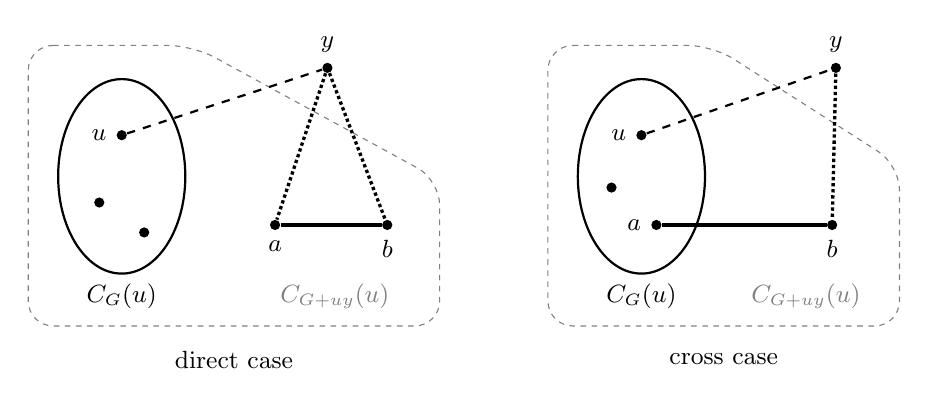
\begin{tikzpicture}[x = 0.95cm, y = 0.95cm,
  vtx/.style = {circle, fill = black, inner sep = 1.3pt},
  rel/.style = {densely dotted, very thick},
  virt/.style = {dashed, thick},
  act/.style = {line width = 1.4pt},
  hull/.style = {gray, dash pattern = on 2pt off 2pt, rounded corners = 9pt},
  lab/.style = {font = \small}]
\begin{scope}
  \draw[hull] (-1.25, 1.75) -- (0.95, 1.75) -- (4.25, -0.05) -- (4.25, -2.0) -- (-1.25, -2.0) -- cycle;
  \draw[thick] (0, 0) ellipse (0.85 and 1.3);
  \node[vtx, label = {[lab]left:$u$}] (u) at (0, 0.55) {};
  \node[vtx] at (-0.3, -0.35) {};
  \node[vtx] at (0.3, -0.75) {};
  \node[lab] at (0, -1.6) {$C_G(u)$};
  \node[vtx, label = {[lab]above:$y$}] (y) at (2.75, 1.45) {};
  \node[vtx, label = {[lab]below:$a$}] (a) at (2.05, -0.65) {};
  \node[vtx, label = {[lab]below:$b$}] (b) at (3.55, -0.65) {};
  \draw[virt] (u) -- (y);
  \draw[rel] (y) -- (a);
  \draw[rel] (y) -- (b);
  \draw[act] (a) -- (b);
  \node[lab, gray] at (2.85, -1.6) {$C_{G + uy}(u)$};
  \node[lab] at (1.5, -2.45) {direct case};
\end{scope}
\begin{scope}[xshift = 6.6cm]
  \draw[hull] (-1.25, 1.75) -- (0.95, 1.75) -- (3.45, 0.15) -- (3.45, -2.0) -- (-1.25, -2.0) -- cycle;
  \draw[thick] (0, 0) ellipse (0.85 and 1.3);
  \node[vtx, label = {[lab]left:$u$}] (u) at (0, 0.55) {};
  \node[vtx, label = {[lab]left:$a$}] (a) at (0.2, -0.65) {};
  \node[vtx] at (-0.4, -0.15) {};
  \node[lab] at (0, -1.6) {$C_G(u)$};
  \node[vtx, label = {[lab]above:$y$}] (y) at (2.6, 1.45) {};
  \node[vtx, label = {[lab]below:$b$}] (b) at (2.55, -0.65) {};
  \draw[virt] (u) -- (y);
  \draw[rel] (y) -- (b);
  \draw[act] (a) -- (b);
  \node[lab, gray] at (2.2, -1.6) {$C_{G + uy}(u)$};
  \node[lab] at (1.1, -2.45) {cross case};
\end{scope}
\end{tikzpicture}

\caption{The credited set of a pair $f = ab$, with the root $u$ and its class $C_G(u)$ (black outline). Dotted lines join pairs of $R_G(u)$. The dashed line is the pair $uy$, which is not added to $G$, and the thick solid line is the added pair $ab$. Left, the direct case: $a, b \in W$ and $y \in R(a) \cap R(b)$. Right, the cross case: $a \in C_G(u)$, $b \in W$, and $y \in R(b)$. In both cases, adding $uy$ would put $a$ and $b$ into the class of $u$ (gray outline), so $G + uy + ab$ is not colorable. Hence every coloring of $G + ab$ gives $y$ the color of $u$.}
\label{fig:high-absorb}
\end{figure}

We next compare $\abs{R_G(u)}$ with two sums, which will appear as the contributions from the direct and cross cases of \eqref{eq:high-credited} to the expected credited logarithmic increment. The comparison is purely combinatorial; it uses the symmetry of $R_G(u)$ and nothing else about colorings.

For a colorable multigraph $G$ on $[n]$ and the fixed root $u$, we define
\begin{equation}\label{eq:high-ain-acr}
\begin{split}
a_1 &= \sum_{(a, b) \in W \times W} \min \biggl( \frac{\abs{R(a) \cap R(b)}}{\abs{C_G(u)}}, 1 \biggr), \\
a_2 &= 2 \bigl( \abs{C_G(u)} - 1 \bigr) \sum_{a \in W} \min \biggl( \frac{\abs{R(a)}}{\abs{C_G(u)}}, 1 \biggr).
\end{split}
\end{equation}
\begin{lemma}\label{lem:high-comb}
For every colorable multigraph $G$ on $[n]$, we have $\abs{R_G(u)} \le 2 a_1 + a_2$.
\end{lemma}

\begin{proof}
We first bound $a_1$ from below. Let $a, b \in W$. Writing the minimum as a sum over the intersection, we have
\[
\min \biggl( \frac{\abs{R(a) \cap R(b)}}{\abs{C_G(u)}}, 1 \biggr) = \sum_{y \in R(a) \cap R(b)} \frac{1}{\max \bigl( \abs{C_G(u)}, \abs{R(a) \cap R(b)} \bigr)},
\]
where both sides vanish if $R(a) \cap R(b) = \emptyset$.

By the symmetry of $R_G(u)$, we have $y \in R(a) \cap R(b)$ if and only if $a, b \in R(y)$. Exchanging the order of summation, we obtain
\[
a_1 = \sum_{y \in W} \sum_{a \in R(y)} \sum_{b \in R(y)} \frac{1}{\max \bigl( \abs{C_G(u)}, \abs{R(a) \cap R(b)} \bigr)} \ge \sum_{y \in W} \sum_{a \in R(y)} \frac{\abs{R(y)}}{\max \bigl( \abs{C_G(u)}, \abs{R(a)} \bigr)},
\]
where in the last step we used $\abs{R(a) \cap R(b)} \le \abs{R(a)}$ and summed over $b \in R(y)$.

The right side is a sum over the pairs $(y, a) \in R_G(u)$. Since $(y, a) \mapsto (a, y)$ is a bijection of $R_G(u)$, the same lower bound holds with the roles of $y$ and $a$ exchanged. Adding the two bounds, we find
\begin{equation}\label{eq:high-comb-1}
2 a_1 \ge \sum_{(y, a) \in R_G(u)} \biggl( \frac{\abs{R(y)}}{\max \bigl( \abs{C_G(u)}, \abs{R(a)} \bigr)} + \frac{\abs{R(a)}}{\max \bigl( \abs{C_G(u)}, \abs{R(y)} \bigr)} \biggr).
\end{equation}

We now split $R_G(u)$ into the pairs $(y, a)$ with $\max(\abs{R(y)}, \abs{R(a)}) \ge \abs{C_G(u)}$ and the remaining pairs. For a pair of the first kind, the summand in \eqref{eq:high-comb-1} is at least $1$. Indeed, by the symmetry of the summand, we may assume that $\abs{R(y)} \ge \abs{R(a)}$. Then $\abs{R(y)} \ge \max(\abs{C_G(u)}, \abs{R(a)})$, and the first fraction in the summand is at least $1$. The bound \eqref{eq:high-comb-1} therefore implies that there are at most $2 a_1$ pairs of the first kind.

It remains to count the pairs $(y, a) \in R_G(u)$ with $\abs{R(y)} < \abs{C_G(u)}$ and $\abs{R(a)} < \abs{C_G(u)}$. When $\abs{C_G(u)} = 1$, there are none, since every pair $(y, a) \in R_G(u)$ satisfies $a \in R(y)$ and hence $\abs{R(y)} \ge 1$. Suppose that $\abs{C_G(u)} \ge 2$.

By symmetry, the vertices $y$ with $(y, a) \in R_G(u)$ form the set $R(a)$, so the number of pairs $(y, a) \in R_G(u)$ with $\abs{R(a)} < \abs{C_G(u)}$ satisfies
\[
\sum_{\substack{a \in W \\ \abs{R(a)} < \abs{C_G(u)}}} \abs{R(a)} \le \abs{C_G(u)} \sum_{a \in W} \min \biggl( \frac{\abs{R(a)}}{\abs{C_G(u)}}, 1 \biggr) \le a_2,
\]
where we used $\abs{C_G(u)} \le 2 (\abs{C_G(u)} - 1)$ in the last step. Adding the two counts gives $\abs{R_G(u)} \le 2 a_1 + a_2$.
\end{proof}

The following lemma is the main step of this section. It bounds $\beta_G(u)$ by the expected credited logarithmic increment when one uniform edge is added to $G$.

\begin{lemma}\label{lem:high-onestep}
Let $G$ be a colorable multigraph on $[n]$, and let $f$ be a uniform pair of $[n]$. Then
\begin{equation}\label{eq:high-onestep}
\beta_G(u) \le \frac{2}{\log 2} \, \E_f \log \biggl( 1 + \frac{\abs{\mathscr{A}_G(f)}}{\abs{C_G(u)}} \biggr),
\end{equation}
where $\E_f$ denotes the expectation with respect to $f$.
\end{lemma}

\begin{proof}
For $z \ge 0$, we have $\log(1 + z) \ge (\log 2) \min(z, 1)$. For $z \in [0, 1]$, this follows from the concavity of $z \mapsto \log(1 + z)$, and for $z > 1$ from its monotonicity. It suffices to show that
\begin{equation}\label{eq:high-onestep-1}
\E_f \min \biggl( \frac{\abs{\mathscr{A}_G(f)}}{\abs{C_G(u)}}, 1 \biggr) \ge \frac{\abs{R_G(u)}}{2 n (n - 1)},
\end{equation}
since the right side of \eqref{eq:high-onestep-1} is bounded below by $\abs{R_G(u)} / (2n^2) = \beta_G(u)/2$.

Since each pair has probability $\binom{n}{2}^{-1} = 2/(n(n - 1))$, we have
\begin{equation}\label{eq:high-onestep-2}
\E_f \min \biggl( \frac{\abs{\mathscr{A}_G(f)}}{\abs{C_G(u)}}, 1 \biggr) = \frac{1}{n(n - 1)} \sum_{\substack{(a, b) \in [n]^2 \\ a \ne b}} \min \biggl( \frac{\abs{\mathscr{A}_G(ab)}}{\abs{C_G(u)}}, 1 \biggr).
\end{equation}
We split the sum in \eqref{eq:high-onestep-2} according to the cases of \eqref{eq:high-credited}. The ordered pairs of distinct vertices of $W$ contribute
\[
a_1 - \sum_{a \in W} \min \biggl( \frac{\abs{R(a)}}{\abs{C_G(u)}}, 1 \biggr),
\]
since the terms of $a_1$ with $a = b$ are $\min(\abs{R(a)} / \abs{C_G(u)}, 1)$.

The ordered pairs with one vertex in $C_G(u)$ and one in $W$ contribute
\[
2 \abs{C_G(u)} \sum_{a \in W} \min \biggl( \frac{\abs{R(a)}}{\abs{C_G(u)}}, 1 \biggr),
\]
since there are $\abs{C_G(u)}$ choices for the vertex in $C_G(u)$ and two orders. The pairs inside $C_G(u)$ contribute zero.

Adding these contributions, we find that the sum in \eqref{eq:high-onestep-2} satisfies
\[
\begin{split}
\sum_{\substack{(a, b) \in [n]^2 \\ a \ne b}} \min \biggl( \frac{\abs{\mathscr{A}_G(ab)}}{\abs{C_G(u)}}, 1 \biggr) &= a_1 + \bigl( 2 \abs{C_G(u)} - 1 \bigr) \sum_{a \in W} \min \biggl( \frac{\abs{R(a)}}{\abs{C_G(u)}}, 1 \biggr)\\
&\ge a_1 + a_2 \ge \frac{1}{2} \abs{R_G(u)},
\end{split}
\]
where we used $2 \abs{C_G(u)} - 1 \ge 2 (\abs{C_G(u)} - 1)$ in the first inequality, and $a_2 \ge 0$ and \cref{lem:high-comb} in the second. Dividing by $n(n - 1)$ gives \eqref{eq:high-onestep-1}.
\end{proof}

The pairs $f$ containing the root compensate for the diagonal terms $a = b$ of $a_1$, which do not correspond to pairs of distinct vertices. Without them, \eqref{eq:high-onestep} would carry an additive error of order $1/n$, and the sum of these errors over the $M$ steps of the process would be of order $\Lambda$.

\section{The potential}\label{sec:high-potential}

We now sum the one-step bound of \cref{lem:high-onestep} over time. The potential $\log \abs{C_{G_m}(u)}$ takes values in $[0, \log n]$. By \cref{lem:high-absorb}, it increases at each step at least by the increment appearing in \eqref{eq:high-onestep}, as long as the graph remains colorable. However, \cref{lem:high-absorb} does not apply at the step at which the graph becomes non-colorable. The increment is still defined at that step, and we bound it using that $C_G(u)$ and $\mathscr{A}_G(f)$ are disjoint subsets of $[n]$.

For each integer $m \ge 0$ with $m < H$, we define
\[
\Phi_m = \log \abs{C_{G_m}(u)}, \qquad \Psi_m = \log \biggl( 1 + \frac{\abs{\mathscr{A}_{G_m}(e_{m + 1})}}{\abs{C_{G_m}(u)}} \biggr).
\]
For $m \ge H$, we set $\Phi_m = \Psi_m = 0$. For $m < H$, the variable $\Psi_m$ is the credited logarithmic increment of $e_{m + 1}$ at $u$.

\begin{theorem}\label{thm:high-potential}
Let $u \in [n]$, let $\tau = \min(H, M)$, and let $\tau_0$ be a stopping time of the filtration $(\cF_m)_{m \ge 0}$ with values in $\{0, 1, 2, \dots\} \cup \{\infty\}$. Then
\begin{equation}\label{eq:high-potential}
\E \sum_{m : \, \tau_0 \le m < \tau} \beta_{G_m}(u) \le \frac{2}{\log 2} \, (\log n) \, \Pp(\tau_0 < \tau).
\end{equation}
\end{theorem}

\begin{proof}
For $m < H$, the multigraph $G_m$ is colorable, so $0 \le \Phi_m \le \log n$ and $\Psi_m \ge 0$. The variable $\Psi_m$ is determined by $G_m$ and $e_{m + 1}$, whether or not $G_{m + 1}$ is colorable.

We first prove a pathwise bound. Let $m + 1 < H$. Then $G_{m + 1} = G_m + e_{m + 1}$ is colorable, and \cref{lem:high-absorb} gives
\begin{equation}\label{eq:high-step}
\abs{C_{G_{m + 1}}(u)} \ge \abs{C_{G_m}(u)} + \abs{\mathscr{A}_{G_m}(e_{m + 1})}, \qquad \text{and hence} \qquad \Psi_m \le \Phi_{m + 1} - \Phi_m.
\end{equation}

Suppose now that $\tau_0 < \tau$. Then $\tau - 1 < H$. The sets $C_{G_{\tau - 1}}(u)$ and $\mathscr{A}_{G_{\tau - 1}}(e_\tau)$ are disjoint subsets of $[n]$, so we have
\[
\Psi_{\tau - 1} = \log \bigl( \abs{C_{G_{\tau - 1}}(u)} + \abs{\mathscr{A}_{G_{\tau - 1}}(e_\tau)} \bigr) - \Phi_{\tau - 1} \le \log n - \Phi_{\tau - 1}.
\]
For $\tau_0 \le m \le \tau - 2$, we have $m + 1 < \tau \le H$, so \eqref{eq:high-step} applies. Telescoping, we obtain
\[
\sum_{m = \tau_0}^{\tau - 1} \Psi_m \le \sum_{m = \tau_0}^{\tau - 2} (\Phi_{m + 1} - \Phi_m) + \log n - \Phi_{\tau - 1} = \log n - \Phi_{\tau_0} \le \log n.
\]

The sum is empty if $\tau_0 \ge \tau$. Together, these cases give
\begin{equation}\label{eq:high-telescope}
\sum_{m : \, \tau_0 \le m < \tau} \Psi_m \le (\log n) \ind \{ \tau_0 < \tau \}.
\end{equation}

Next, we compare the expectations. For $0 \le m < M$, we define $I_m$ by
\[
I_m = \ind \{ \tau_0 \le m < \tau \}.
\]
Since $\tau_0$ is a stopping time and, for $m < M$, the event $\{ m < \tau \}$ is the event that $G_m$ is colorable, the variable $I_m$ is $\cF_m$-measurable.

The pair $e_{m + 1}$ is uniform and independent of $\cF_m$. On the event $\{ m < H \}$, the conditional expectation of $\Psi_m$ given $\cF_m$ is the expectation in \eqref{eq:high-onestep} with $G = G_m$. Using \cref{lem:high-onestep} and $I_m \le \ind \{ m < H \}$, we obtain
\[
\E \bigl[ I_m \beta_{G_m}(u) \bigr] \le \frac{2}{\log 2} \, \E \bigl[ I_m \, \E [ \Psi_m \mid \cF_m ] \bigr] = \frac{2}{\log 2} \, \E \bigl[ I_m \Psi_m \bigr].
\]
Since $\tau \le M$, summing over $0 \le m < M$ and using \eqref{eq:high-telescope}, we conclude that
\[
\begin{split}
\E \sum_{m : \, \tau_0 \le m < \tau} \beta_{G_m}(u) &= \sum_{m = 0}^{M - 1} \E \bigl[ I_m \beta_{G_m}(u) \bigr] \le \frac{2}{\log 2} \, \E \sum_{m : \, \tau_0 \le m < \tau} \Psi_m\\
&\le \frac{2}{\log 2} \, (\log n) \, \Pp(\tau_0 < \tau).
\end{split}
\]
This completes the proof.
\end{proof}

The passage from the one-step bound to \eqref{eq:high-potential} is a standard compensator argument, in the spirit of the drift bounds for hitting and occupation times in \cite[Sections~2--3]{hajek1982hitting}. A related use of a bounded monotone potential to control occupation, retaining terminal increments, appears in \cite[Lemmas~2.2 and~4.1]{openai2026linear}. Here the potential is the logarithm of a frozen-class size, and the input specific to colorings is \cref{lem:high-onestep}.

\begin{remark}\label{rem:high-killing}
The proof of \cref{thm:high-potential} credits the edge $e_\tau$ with the increment $\Psi_{\tau - 1}$, which is defined from $G_{\tau - 1}$ and $e_\tau$ even when $G_\tau$ is not colorable. If $\tau = H$, this edge is the final edge; if $\tau = M < H$, it is the edge at the cap. Correspondingly, the average in \cref{lem:high-onestep} runs over all pairs $f$, including those for which $G + f$ is not colorable. This cannot be avoided, as the following example shows. Let $q = 3$, let $n \ge 7$ with $n - 1$ divisible by $3$, and let the root be $u = n$. Let $G$ consist of the triangle on the vertices $1, 2, 3$, of $(n - 4)/3$ vertices joined to $2$ and $3$, of $(n - 4)/3$ vertices joined to $1$ and $3$, of $(n - 4)/3$ vertices joined to $1$ and $2$, and of the edge joining $u$ to $3$. In every coloring, the triangle receives three distinct colors, and every other vertex except $u$ receives the color of the vertex of the triangle to which it is not joined. Thus $G$ has three frozen classes besides $\{u\}$, each of size $(n - 1)/3$. For $i \in \{1, 2, 3\}$, we let $C_i$ denote the frozen class that contains the vertex $i$. The root can take the color of $C_1$ or that of $C_2$, so $C_G(u) = \{u\}$, and \eqref{eq:high-R} shows that $R_G(u) = (C_1 \times C_2) \cup (C_2 \times C_1)$. Therefore
\[
\beta_G(u) = \frac{2 (n - 1)^2}{9 n^2},
\]
which tends to $2/9$ as $n \to \infty$.

On the other hand, a pair $f$ with $\mathscr{A}_G(f) \ne \emptyset$ either lies inside $C_1$ or inside $C_2$, in which case $G + f$ is not colorable, or joins $u$ to a vertex of $C_1 \cup C_2$. There are $2(n - 1)/3$ pairs of the last kind, each with a credited set of size $(n - 1)/3$, so
\[
\E_f \biggl[ \log \biggl( 1 + \frac{\abs{\mathscr{A}_G(f)}}{\abs{C_G(u)}} \biggr) \ind \{ G + f \text{ is colorable} \} \biggr] = \binom{n}{2}^{-1} \frac{2(n - 1)}{3} \log \frac{n + 2}{3} \le \frac{4 \log n}{3n}.
\]
Let $C, C' \ge 0$ be constants independent of $n$. Then a bound of the form
\[
\beta_G(u) \le C \, \E_f \biggl[ \log \biggl( 1 + \frac{\abs{\mathscr{A}_G(f)}}{\abs{C_G(u)}} \biggr) \ind \{ G + f \text{ is colorable} \} \biggr] + C' \frac{\log n}{n},
\]
fails for large $n$. However, this does not contradict \cref{thm:high-potential}. About a third of all pairs lie inside one of the classes $C_1$, $C_2$, $C_3$, and $\kappa(G)$ is close to $1/3$. By \cref{lem:pre-lifetime}(c) and (d), on the event $\{G_m = G\}$, the conditional expectation of $H - m$ given $\cF_m$ is $r(G) \le 1/\kappa(G)$, which is bounded.
\end{remark}

We apply \cref{thm:high-potential} at the time at which the root reaches a given degree.

\begin{corollary}\label{cor:high-degree}
For all $u \in [n]$ and all integers $j \ge 1$,
\begin{equation}\label{eq:high-degree}
\sum_{m = 0}^{M - 1} \E \bigl[ \ind \{ \deg_{G_m}(u) \ge j \} \, \beta_{G_m}(u) \bigr] \le \frac{2}{\log 2} \, (\log n) \biggl( \frac{2 e \Lambda}{j} \biggr)^j.
\end{equation}
\end{corollary}

\begin{proof}
We may assume that $M \ge 1$, since otherwise the left side vanishes. We set $\tau = \min(H, M)$ and let $\tau_0$ denote the first time $m \ge 0$ such that $\deg_{G_m}(u) \ge j$, with $\tau_0 = \infty$ if there is no such time. Then $\tau_0$ is a stopping time.

Since degrees do not decrease in $m$, we have $\deg_{G_m}(u) \ge j$ if and only if $\tau_0 \le m$. Further, $\beta_{G_m}(u) = 0$ for $m \ge H$. The left side of \eqref{eq:high-degree} is the left side of \eqref{eq:high-potential}. By \cref{thm:high-potential}, it is bounded by $(2 / \log 2) (\log n) \Pp(\tau_0 < \tau)$.

On the event $\{ \tau_0 < \tau \}$, we have $\tau_0 \le M - 1$ and hence $\deg_{G_{M - 1}}(u) \ge j \ge 1$; in particular, this event is empty if $M = 1$. Suppose that $M \ge 2$. Recall that $\deg_{G_{M - 1}}(u)$ has the law $\Bin(M - 1, 2/n)$. Using \cref{lem:pre-tails}(a) and $M - 1 \le \Lambda n$, we obtain
\[
\Pp(\tau_0 < \tau) \le \Pp \bigl( \Bin(M - 1, 2/n) \ge j \bigr) \le \biggl( \frac{2 e (M - 1)}{n j} \biggr)^j \le \biggl( \frac{2 e \Lambda}{j} \biggr)^j,
\]
which completes the proof.
\end{proof}

\section{Combining the estimates}\label{sec:high-main}

We now combine \cref{prop:high-descent}, \cref{lem:high-deletion}(b), and \cref{cor:high-degree}.

\begin{theorem}\label{thm:high-main}
Let $n \ge 3$ be such that $w_0 \ge K$, where $K$ and $w_0$ are given by \eqref{eq:high-params}. Then
\begin{equation}\label{eq:high-main}
\begin{split}
&\Pp \Bigl( H \le M, \ \max_{v \in e_H} \deg_\Gamma(v) > D_n \Bigr)\\
&\qquad \le \frac{8}{3} \, 4^{-(D_n + 1 - w_0)} + \frac{32 \Lambda}{3 \log 2} \biggl( \frac{n}{n - 1} \biggr)^2 \frac{\log n}{w_0 - K + 2} \biggl( \frac{2 e \Lambda}{w_0} \biggr)^{w_0}.
\end{split}
\end{equation}
Further, there exists $n_0$, depending only on $\Lambda$, such that for all $n \ge n_0$ the right side of \eqref{eq:high-main} is at most $(\log n)^{-3/2}$. In particular, for all $n \ge n_0$ and all integers $0 \le L' \le U' \le M$,
\begin{equation}\label{eq:high-main-window}
\Pp \Bigl( L' < H \le U', \ \min_{v \in e_H} \deg_\Gamma(v) > D_n \Bigr) \le (\log n)^{-3/2}.
\end{equation}
\end{theorem}

\begin{proof}
We bound the pivotal sum in \eqref{eq:high-descent}. Fix $u \in [n]$ and let $w_0 + 1 \le j \le m \le M - 1$. Then $j \ge K + 1$, so that \eqref{eq:high-deletion-piv} applies, and $j - K + 1 \ge w_0 - K + 2$. Using \eqref{eq:high-deletion-piv} and $m \le M \le \Lambda n$, we find
\[
\E \kappa_j^{\rm piv}(G_m) \le \frac{2 \Lambda}{w_0 - K + 2} \biggl( \frac{n}{n - 1} \biggr)^2 \E \bigl[ \ind \{ \deg_{G_{m - 1}}(u) = j - 1 \} \, \beta_{G_{m - 1}}(u) \bigr].
\]

For fixed $m$, the events $\{ \deg_{G_{m - 1}}(u) = j - 1 \}$ with $w_0 + 1 \le j \le m$ are disjoint and contained in $\{ \deg_{G_{m - 1}}(u) \ge w_0 \}$. Exchanging the order of summation, we obtain
\[
\begin{split}
\sum_{j = w_0 + 1}^{M - 1} \sum_{m = j}^{M - 1} \E \bigl[ \ind \{ \deg_{G_{m - 1}}(u) = j - 1 \} \, \beta_{G_{m - 1}}(u) \bigr] &\le \sum_{m = 0}^{M - 1} \E \bigl[ \ind \{ \deg_{G_m}(u) \ge w_0 \} \, \beta_{G_m}(u) \bigr]\\
&\le \frac{2}{\log 2} \, (\log n) \biggl( \frac{2 e \Lambda}{w_0} \biggr)^{w_0},
\end{split}
\]
where the last inequality is \cref{cor:high-degree} with $j = w_0 \ge 1$.

Inserting the last two displays into \eqref{eq:high-descent} and using $(8/3) \cdot 2 \Lambda \cdot (2 / \log 2) = 32 \Lambda / (3 \log 2)$, we obtain \eqref{eq:high-main}.

We now show that the right side of \eqref{eq:high-main} is small for large $n$. We have
\[
D_n + 1 - w_0 \ge \frac{D_n}{2} + 1 \ge \frac{(\log n)^{1/4}}{2}, \qquad w_0 \ge \frac{D_n - 1}{2} \ge \frac{(\log n)^{1/4}}{2} - 1,
\]
where we used $D_n \ge (\log n)^{1/4} - 1$ and $(D_n - 1)/2 \le w_0 \le D_n/2$.

By the first bound, the first term in \eqref{eq:high-main} is bounded by $(8/3) \, 2^{-(\log n)^{1/4}}$. The second implies that $w_0 \to \infty$. We take $n$ large enough that $w_0 \ge \max(K, 2 e^2 \Lambda)$. Then $\log(w_0 / (2 e \Lambda)) \ge 1$, which gives
\[
\biggl( \frac{2 e \Lambda}{w_0} \biggr)^{w_0} = \exp \biggl( - w_0 \log \frac{w_0}{2 e \Lambda} \biggr) \le e^{-w_0} \le e^{1 - (\log n)^{1/4} / 2}.
\]
Using also $w_0 - K + 2 \ge 2$ and $(n/(n - 1))^2 \le 9/4$, we bound the second term in \eqref{eq:high-main} by $(12 e \Lambda / \log 2) (\log n) e^{-(\log n)^{1/4} / 2}$. As $x^{5/2} e^{-x^{1/4}/2} \to 0$ and $x^{3/2} 2^{-x^{1/4}} \to 0$ as $x \to \infty$, each term is bounded by $(\log n)^{-3/2} / 2$ for all large $n$, with a threshold that depends only on $\Lambda$.

Finally, let $0 \le L' \le U' \le M$. The event in \eqref{eq:high-main-window} is contained in the event in \eqref{eq:high-main}, since $H \le U' \le M$ on this event and the minimum of the two degrees is at most their maximum. This gives \eqref{eq:high-main-window}.
\end{proof}

\begin{remark}\label{rem:high-q2}
For $q = 2$, the conclusion of this section has a short direct proof. Indeed, we now show that $\kappa_j^{\rm piv} = 0$ for all $j > K$ when $q = 2$. Let $G$ be a colorable multigraph and let $u \sim_G v$ with $u \ne v$. A connected bipartite multigraph has exactly two colorings with two colors, which differ by exchanging the colors, and different components can be colored independently. This implies that $u$ and $v$ lie in the same component of $G$, at even distance. Let $e$ be an occurrence at $u$ such that $u$ and $v$ are still connected in $G - e$. Then they are at even distance in $G - e$ as well, since every path in $G - e$ is a path in the bipartite multigraph $G$, and therefore $u \sim_{G - e} v$. A pivotal occurrence at $u$ is thus an occurrence of a pair that lies on every path from $u$ to $v$. We fix one such path without repeated vertices. Its only edge at $u$ is its first edge, so every pivotal occurrence at $u$ is an occurrence of this pair. Since a pair with a pivotal occurrence has multiplicity one, at most one occurrence at $u$ is pivotal for $(u, v)$. If $\deg_G(u) = j > K$, then at least $j - 1 \ge K$ occurrences at $u$ are non-pivotal, and $\kappa_j^{\rm piv}(G) = 0$. If $w_0 \ge K$, all pivotal terms in \cref{prop:high-descent} then vanish, which leaves the bound $(8/3) \, 4^{-(D_n + 1 - w_0)}$ without the potential argument. In particular, the proof of \cref{thm:high-main} does not use $q \ge 3$.
\end{remark}
